\section{数据下载}
\subsection{安装下载工具}
\begin{frame}
    \frametitle{下载安装包}
    打开项目位置, 下载0.9的安装包

    \url{https://github.com/xiaoke0O/LAADS-Order-Tool/releases}

    \begin{annotationimage}{width=\linewidth}{images/2B.1Release}
        \draw[red,very thick](0.24,0.58) rectangle (0.48,0.63);
    \end{annotationimage}
\end{frame}
\begin{frame}
    \frametitle{创建虚拟环境,以Conda为例}
    打开Conda 的命令窗口,输入以下命令并回车

    conda create -n run-laadsTool python=3.8 setuptools=52 -y
\end{frame}
\begin{frame}
    \frametitle{激活虚拟环境}
    输入激活命令,激活该新建的环境
    \begin{annotationimage}{width=\linewidth}{images/2B.2激活环境}
        \draw[red,very thick](0.23,0.38) rectangle (0.54,0.43);
        \draw[red,very thick](0.01,0.29) -- (0.16,0.29);
    \end{annotationimage}
\end{frame}
\begin{frame}
    \frametitle{使用pip 安装}

    继续在窗口输入pip install ,然后用鼠标将下载的安装包拖进来(就会自动输入安装包的
    路径),回车以安装
    \begin{annotationimage}{width=\linewidth}{images/2B.3安装}
        \draw[red,very thick](0.33,0.3) -- (0.96,0.3);
        \draw[red,very thick](0.01,0.25) -- (0.16,0.25);
    \end{annotationimage}
\end{frame}
\begin{frame}
    \frametitle{运行laadsOrderTool}
    安装成功后,继续输入laadsOrderTool,回车以运行
    \begin{annotationimage}{width=\linewidth}{images/2B.4运行}
        \draw[red,very thick](0.01,0.43) -- (0.24,0.43);
        \draw[red,very thick](0.33,0.12) -- (0.48,0.12);
    \end{annotationimage}
\end{frame}
\begin{frame}
    \frametitle{主界面}
    如果显示了了主界面,说明安装成功
    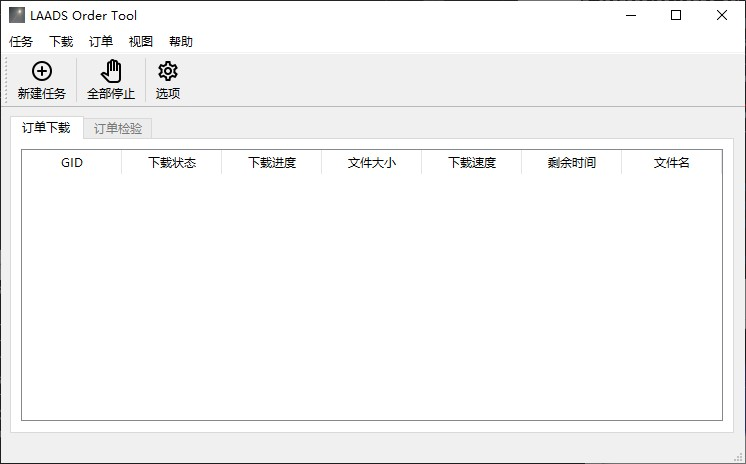
\includegraphics[width=\linewidth]{images/2B.5主界面.jpg}
\end{frame}
\subsection{获取授权Token}
\begin{frame}
    \frametitle{}
    在LAADS主页,点Profile,点击Generate Token
    \begin{annotationimage}[grid]{width=\linewidth}{images/8.登录完成}
        \draw[red,very thick](0.89,0.84) rectangle (0.98,0.88);
    \end{annotationimage}


\end{frame}
为了保护用户的用户名和密码不被泄露,现在使用Token进行用户的下载权限识别


\subsection{导入订单下载}

\subsection{自动校验订单}